%===================================== CHAP 5 =================================

\chapter{Experimental testing}
This chapter present the results from the tests that were performed. Here the goal of the tests were to test the performance of the Ublox LEA M8T, compare the performance of the \acrfull{rtklib} with the Piksi alternative, and to compare the real time estimate from both system with the post-processed solution. The raw \gls{gnss} data from the Ubloxs are used to compute the post processed solution. The comparison test was performed with the Piksi and the Ublox connected to the same antenna at both the rover and the base station. Hence the deviation in the position estimate is limited to the receivers. All position and velocity data is given in the \gls{ned} frame, however altitude is only used for the flight test.
\section{Performance testing of UAV Position System}
The experimental test was split in two independent test, one where the X8 \gls{uav} was carried around on a open field to test the performance of the position system in a more controlled environment, and a second test where the \gls{uav} was flying by means of pilot control. The goal of the first test was to log data from both \gls{rtk-gps} systems in optimal condition. The objective of the second test was to test the systems in a more realistic environment for application in an automatic net landing system. 


\subsection{Test 1: Test of the RTK-GPS navigation system}
The first test was repeated twice where the results from both runs are presented. Both tests were performed on the same day, which was cloudless and at a time with good satellite constellation geometry. The raw data from the Ublox receivers were post processed with \gls{rtklib}, which is assumed more accurate than real time processed data. Therefore an estimate of error is defined as:
\begin{equation}
e(t) = p_r(t) - p_p(t)
\end{equation}
where $p_r(t)$ and $p_p(t)$ is defined as the position solution from the real time system and the position solution from the post processed solution respectfully. The error estimate, $e(t)$, is used as a measure on the performance of the position estimate relative to the assumed more accurate post-processed estimate. In order to compare the different time-series the position data was synchronized with each other. From the error the cumulative standard deviation was calculated using the matlab function "std".
\section{Test 1 - Walk test 1}

In the first session of the test the \gls{uav} was carried around on a open field, and later placed exactly on the same place where it started. As expected both systems provided a position estimate with fixed integer ambiguity solution that followed the true path, and further confirms that both system performed in a similar manner. Therefore both systems are suitable for further comparison of position estimation in a flying test.
Figure \ref{figure:xywalk1} shows a North East plot of how the walk was. The plot contain only the fixed solution from both the piksi and rtklib. 
\begin{figure}[H]
	\centering
		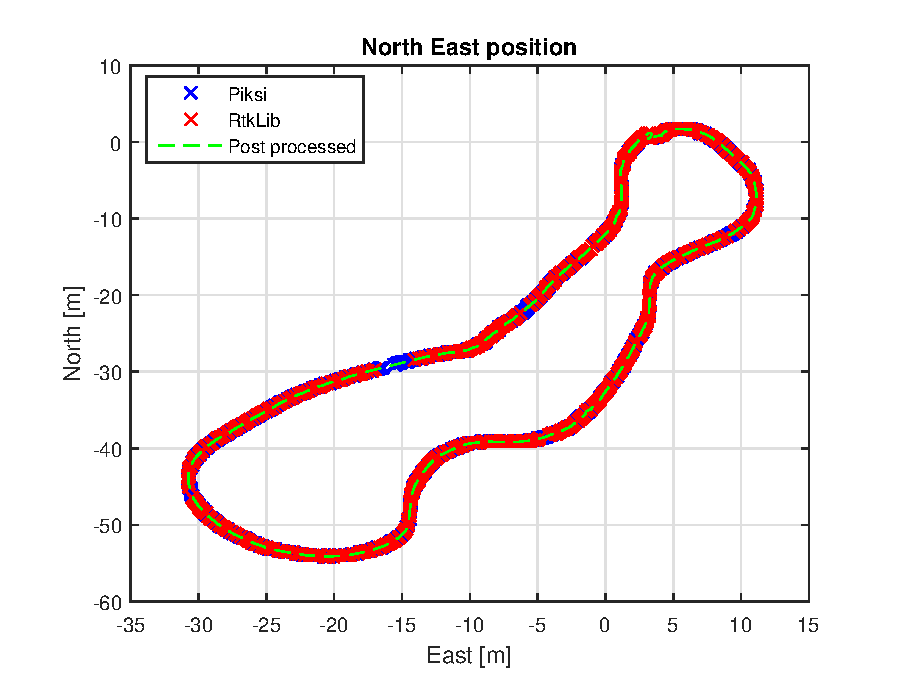
\includegraphics[width=0.7\textwidth]{figs/plots/xywalk1.eps}
		\caption{The North/East position during the first test}
		\label{figure:xywalk1}
\end{figure}
~\\
\paragraph{Integer ambiguity solution and position error}~\\

Figure \ref{figure:DownAndAmbwalk1} shows the Down position, as well as how the integer ambiguity solution was during the experiment. As seen in the figure both the Piksi and \gls{rtklib} manage to keep there fixed solution. The position solution from both the Piksi and \gls{rtklib} agrees with the post processed solution. 
\begin{figure}[H]
	\centering
		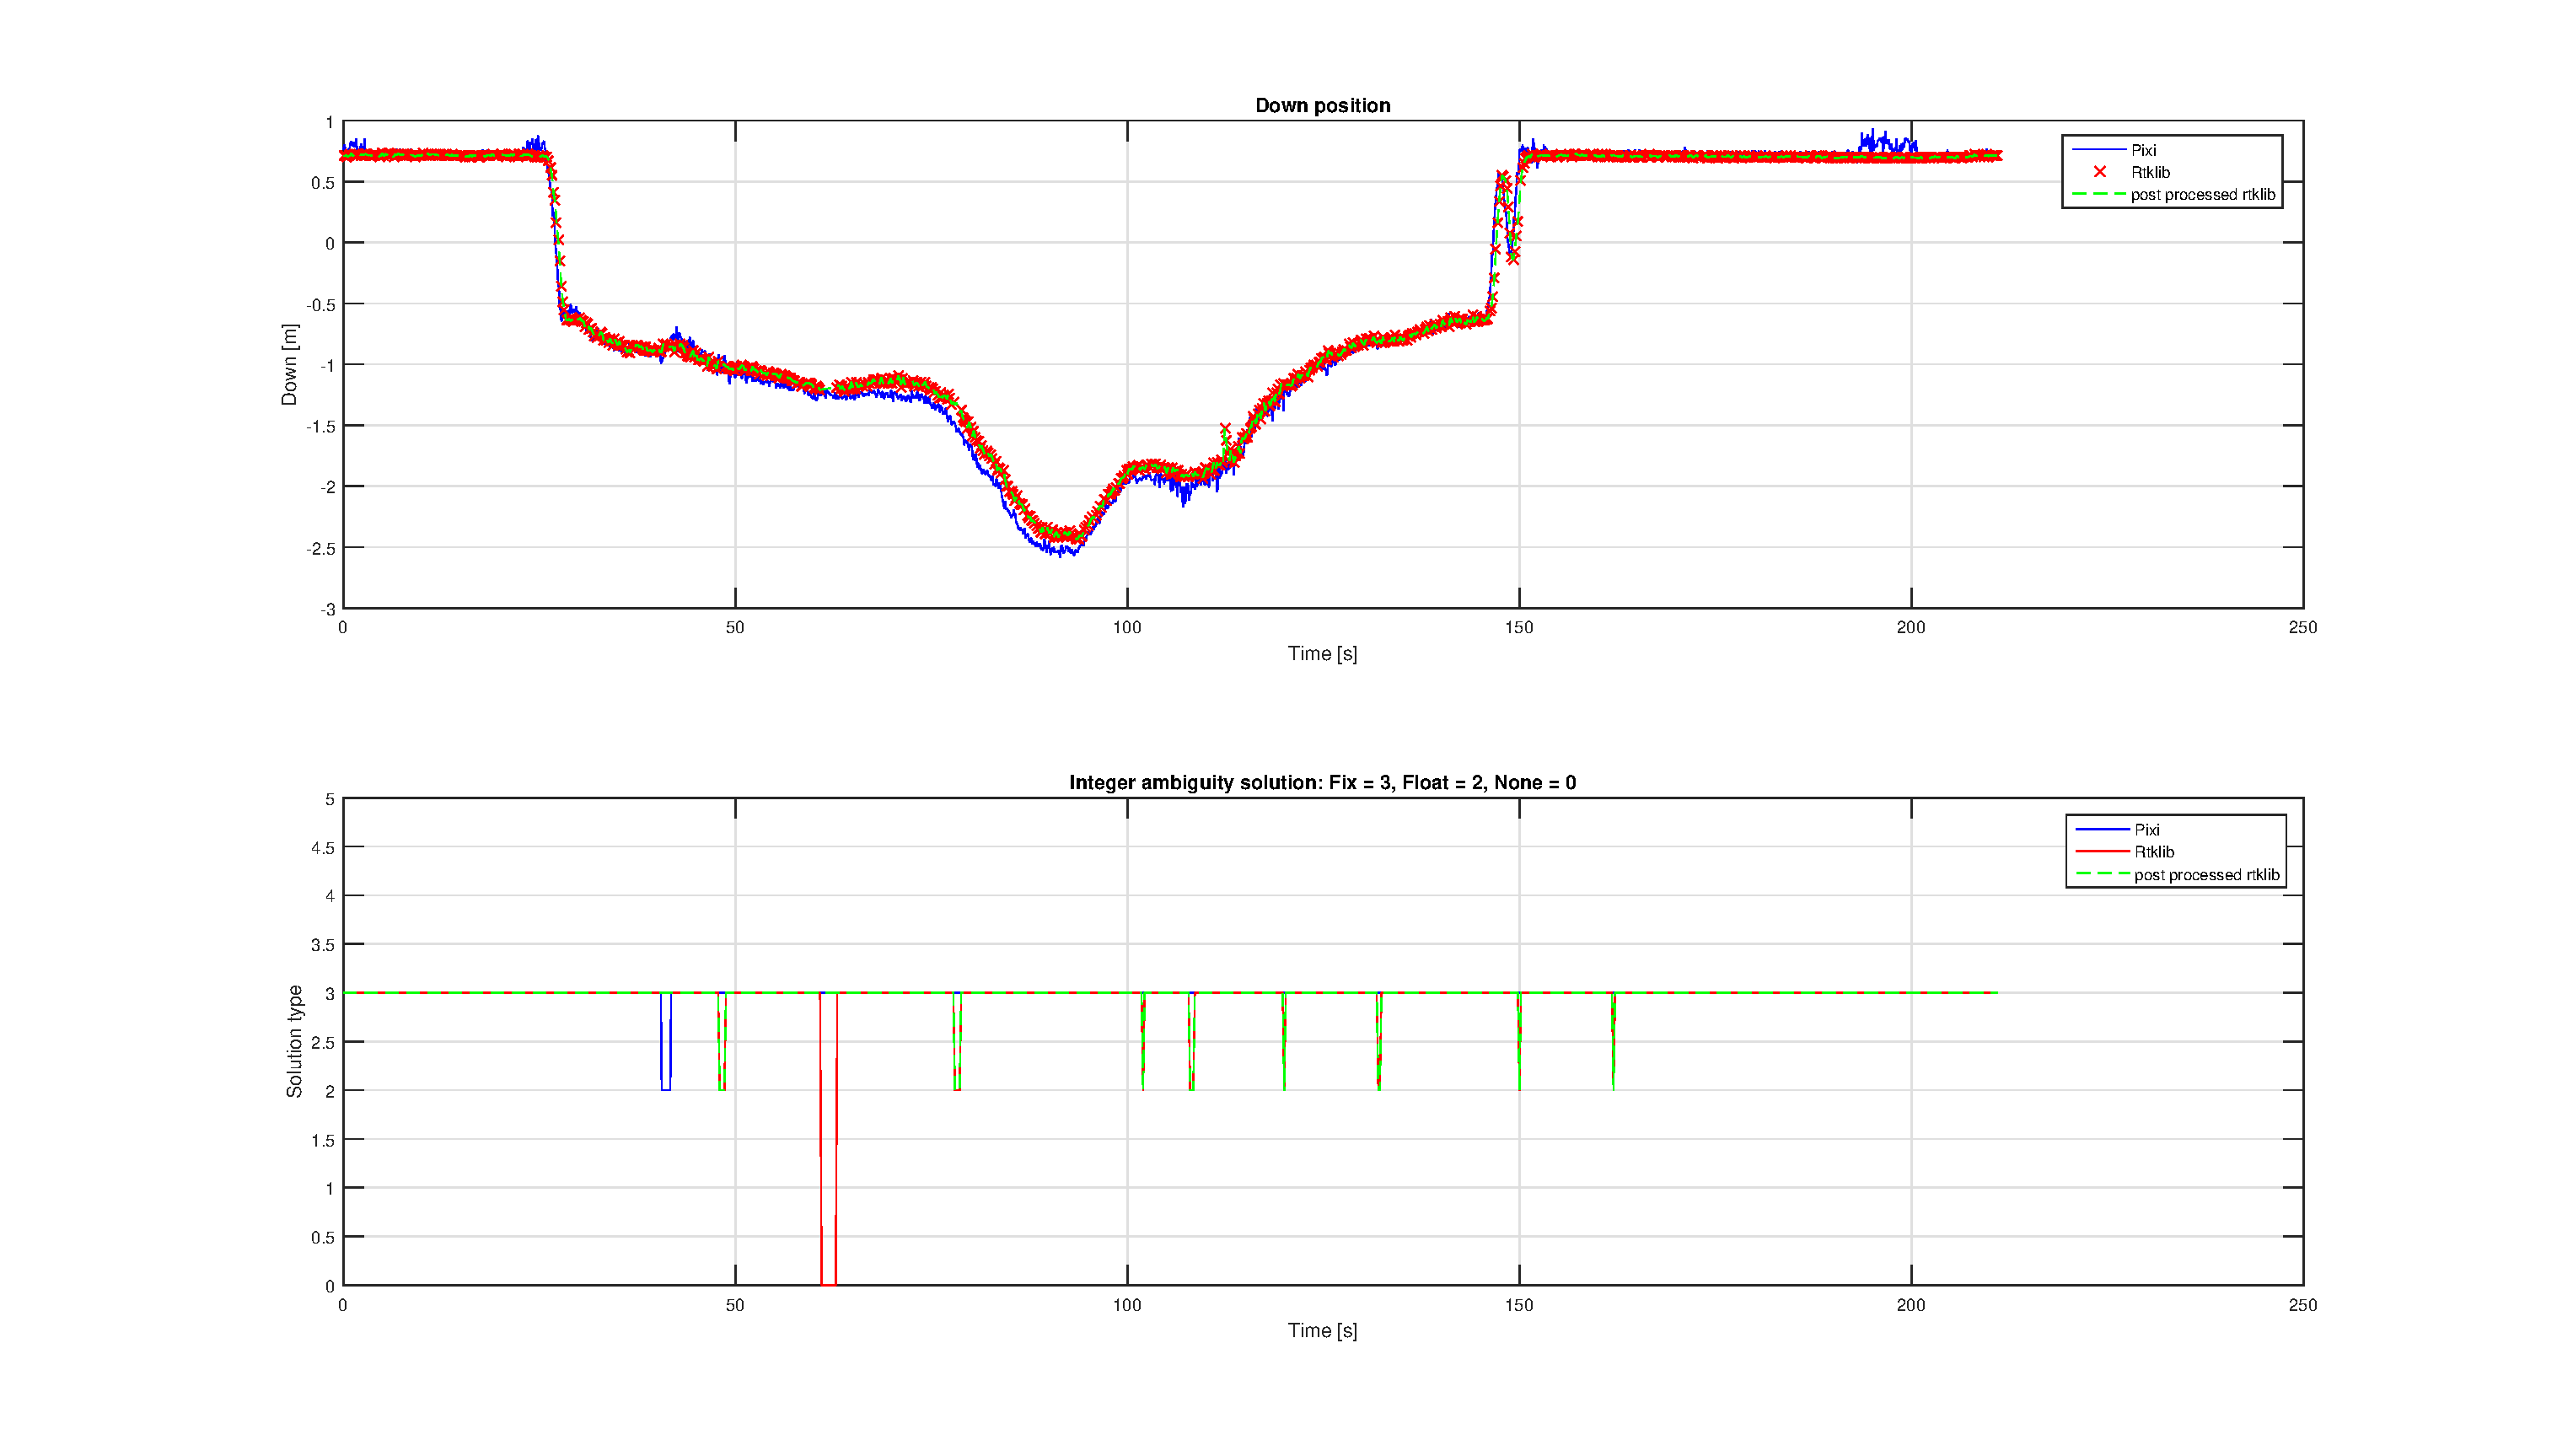
\includegraphics[width=0.7\textwidth]{figs/plots/downWalk1.eps}
		\caption{The Down position and integer ambiguity solution during the first test}
		\label{figure:DownAndAmbwalk1}
\end{figure}
As seen in figure \ref{figure:xywalk1} the difference between the solutions are quite small, which is confirmed in the error plot shown in figure \ref{figure:errorRTKwalk1} and \ref{figure:errorPiksiwalk1}
\begin{figure}[H]
	\centering
		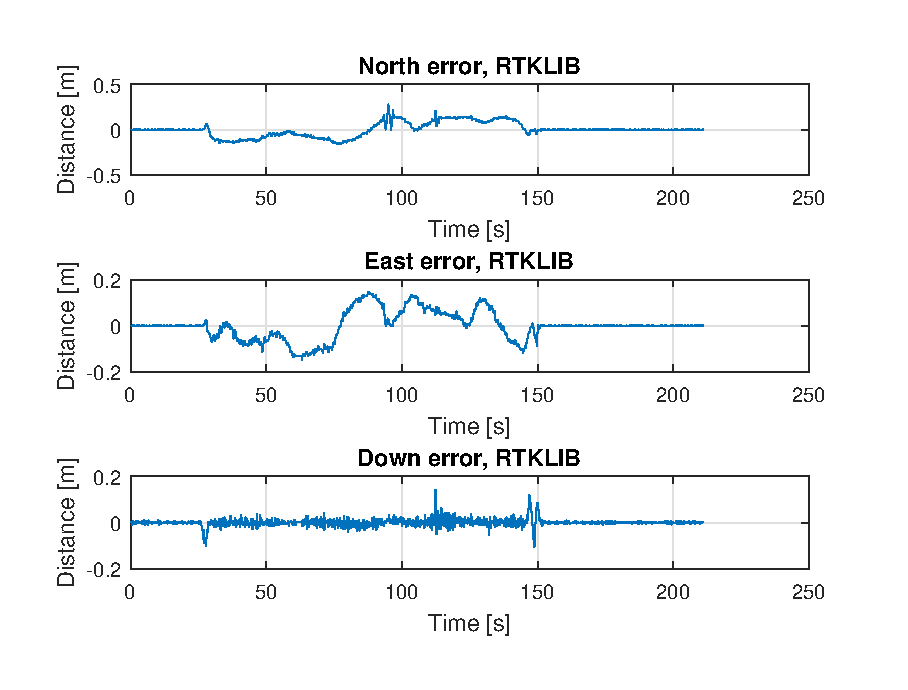
\includegraphics[width=0.7\textwidth]{figs/plots/errorRtklibWalk1.eps}
		\caption{The error from \gls{rtklib}}
		\label{figure:errorRTKwalk1}
\end{figure}
\begin{figure}[H]
	\centering
		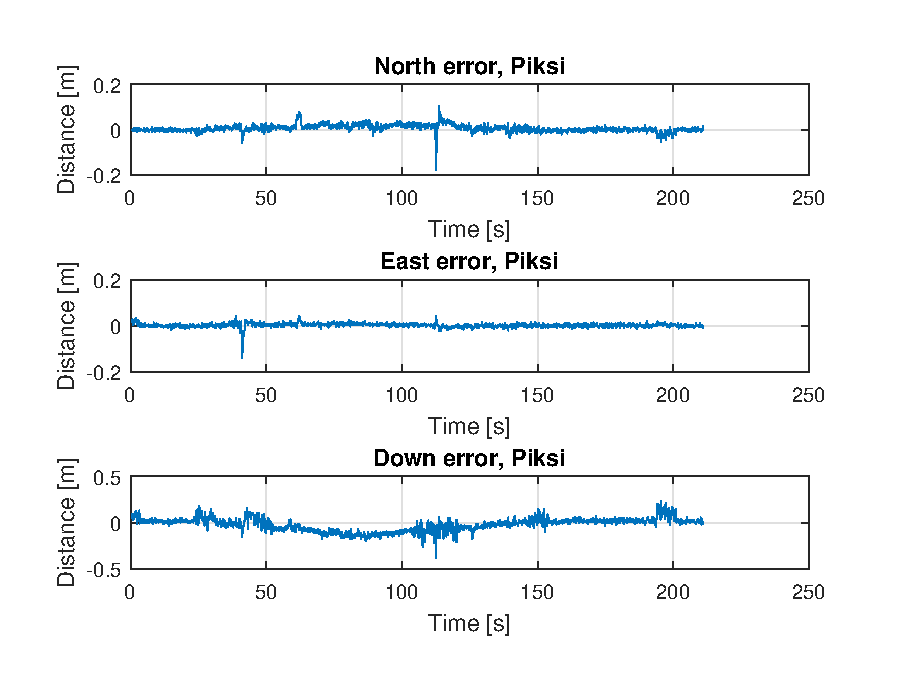
\includegraphics[width=0.7\textwidth]{figs/plots/errorPiksiWalk1.eps}
		\caption{The error from Piksi}
		\label{figure:errorPiksiwalk1}
\end{figure}
\paragraph{Cumulative standard deviation}~\\

The cumulative standard deviation for the error from both the Piksi and \gls{rtklib} indicate that the estimate has a high precision, as seen in figure \ref{figure:stdPiksi} and \ref{figure:stdRTK}. The high precision in the navigation system is critical in a automatic net landing system require to be able to follow a accurate landing path.
\begin{figure}[H]
	\centering
		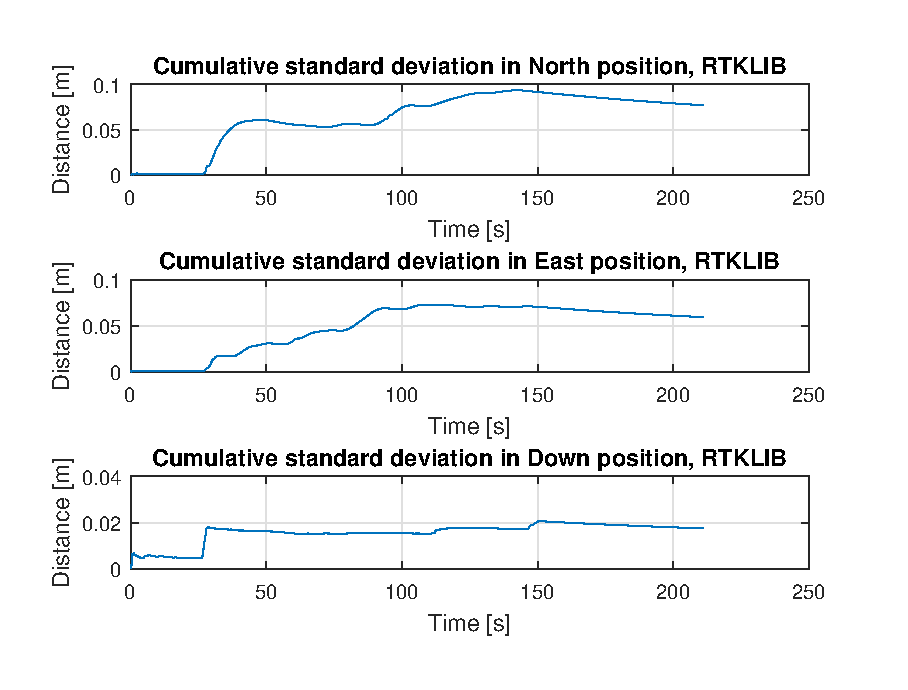
\includegraphics[width=0.7\textwidth]{figs/plots/stdRtklibWalk1.eps}
		\caption{The cumulative standard deviation from \gls{rtklib}}
		\label{figure:stdRTK}
\end{figure}
\begin{figure}[H]
	\centering
		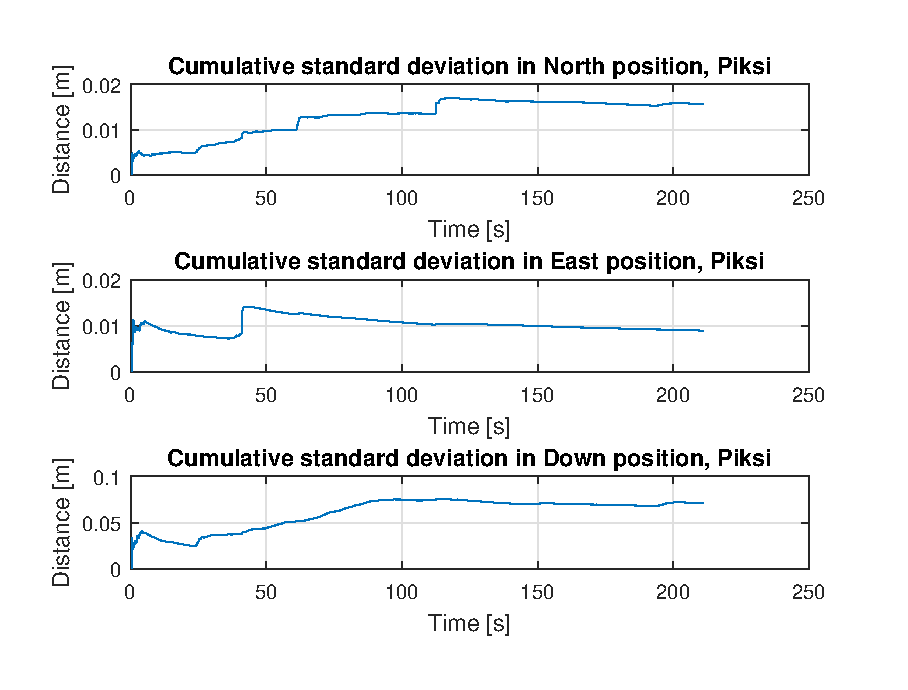
\includegraphics[width=0.7\textwidth]{figs/plots/stdPiksiWalk1.eps}
		\caption{The cumulative standard deviation from Piksi}
		\label{figure:stdPiksi}
\end{figure}
\paragraph{Velocity}~\\

Both the Piksi and \gls{rtklib} agrees to the same estimate in North and East velocity, as seen in figure \ref{figure:VelocityWalk1}. However the Down velocity from \gls{rtklib} is more noisy then the Piksi. The noisy behaviour could be because the \gls{uav} was carried around.
\begin{figure}[H]
	\centering
		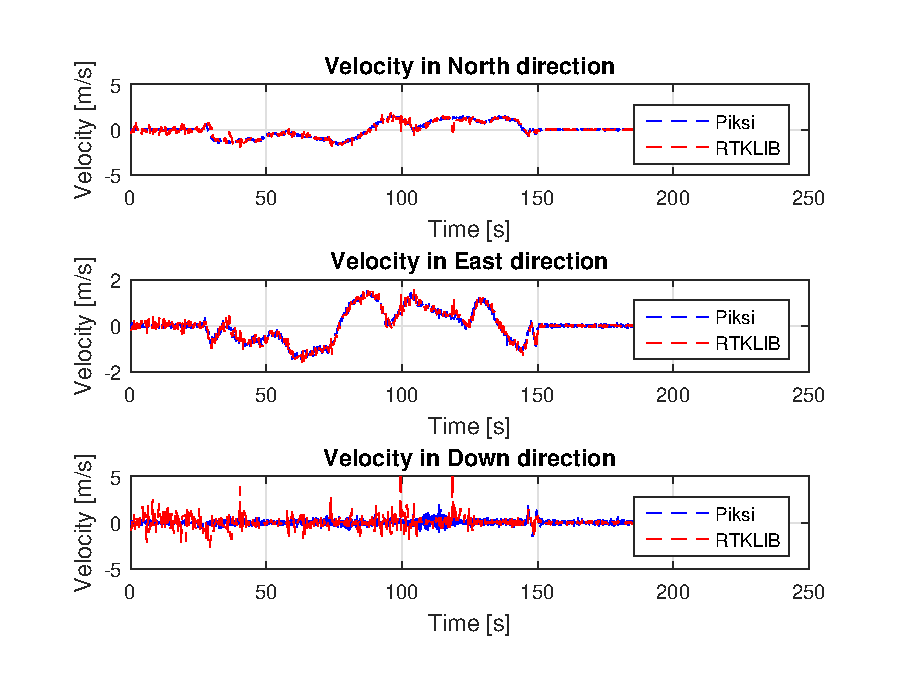
\includegraphics[width=0.7\textwidth]{figs/plots/velocityWalk1.eps}
		\caption{The velocity from the first test}
		\label{figure:VelocityWalk1}
\end{figure}
\paragraph{Satellite tracking}~\\

The different receivers used in \gls{rtklib} and Piksi was not able to track the same satellites at all time. Figure \ref{figure:NumSatWalk1} shows that the Ublox LEA M8T receivers connected to \gls{rtklib} managed to track more satellites then the receiver used in Piksi. 
\begin{figure}[H]
	\centering
		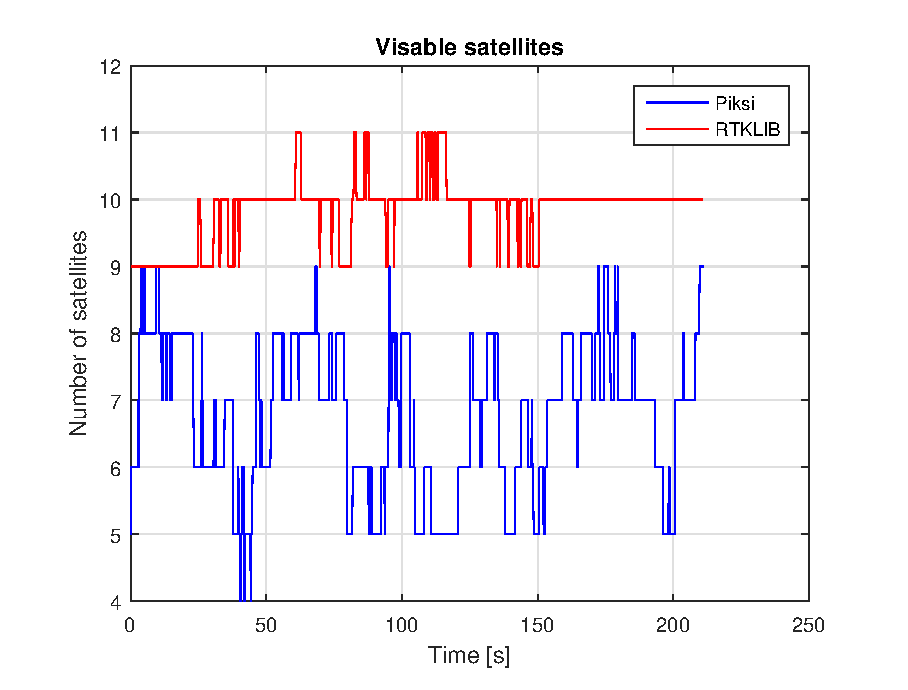
\includegraphics[width=0.7\textwidth]{figs/plots/numSatWalk1.eps}
		\caption{Number of visible satellites in the first test}
		\label{figure:NumSatWalk1}
\end{figure}
\paragraph{Accuracy for stationary position estimate}~\\

The position estimate of the rover is a relative position in reference to the base station. Due to the fact that the position of the base station is calculated with a single receiver with one frequency, there will be introduced a bias in the position estimate. Figure \ref{figure:enhancedxywalk1} shows the North, East position of the the first walk. The true position is exactly the same, however in the figure the distance is approximately $5-10cm$. The distance from the base station to the estimated start and stop position was calculated to be $3.3553m$ and $3.2914m$ respectfully. The measured distance was approximately $3.3m$. That gives an initial error off $0.02m$. The true Down position was measured to approximately $0.78m$. \gls{rtklib} had a initial Down position of $0.7096m$, and stop position at $0.7155m$. This five a initial error of $-0.704m$ and stop error of $-0.0645m$ for \gls{rtklib}. For Piksi the initial Down position was $0.7630m$ and stop position of $0.721m$, which gives and error of $-0.0170m$ and $-0.0590m$ for initial and stop position respectfully. This gives an accuracy level at centimetre level at stationary condition. 
\begin{figure}[H]
	\centering
		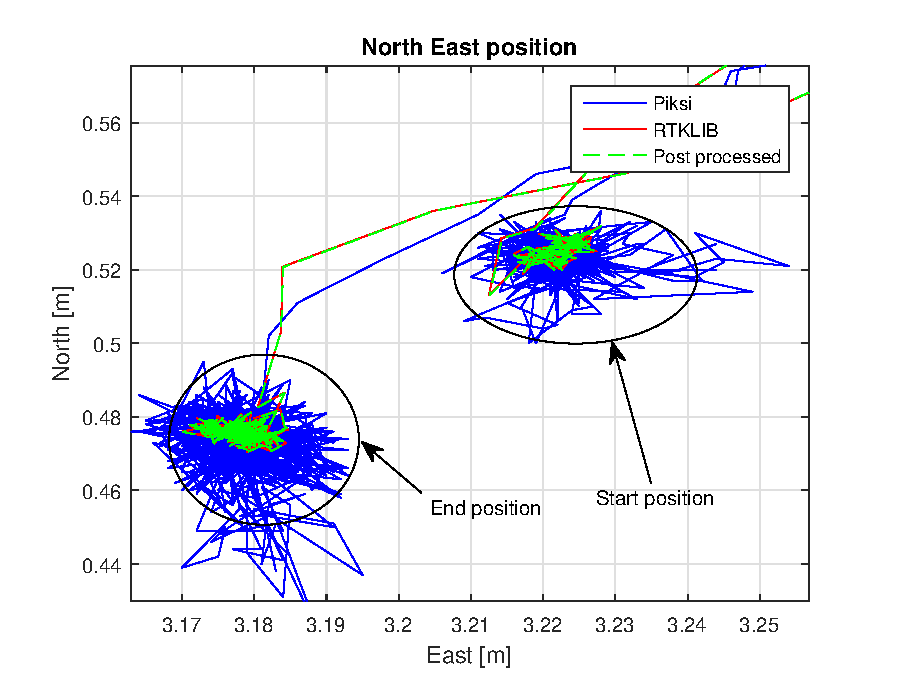
\includegraphics[width=0.7\textwidth]{figs/plots/enhancedxywalk1.eps}
		\caption{Enhanced North/East plot from the first test}
		\label{figure:enhancedxywalk1}
\end{figure}
\paragraph{Time delay}~\\

The position estimate from \gls{rtklib} is delayed in comparison to the solution from the Piksi. Figure \ref{figure:DownDelay} shows that both the post processed solution and the real time solution is delay by $0.5$ secounds compared to the Piksi. This could be how \gls{rtklib} resolve the millisecond in \acrfull{tow}, and may not be seen as an extra delay seen from the control systems perspective.
\begin{figure}[H]
	\centering
		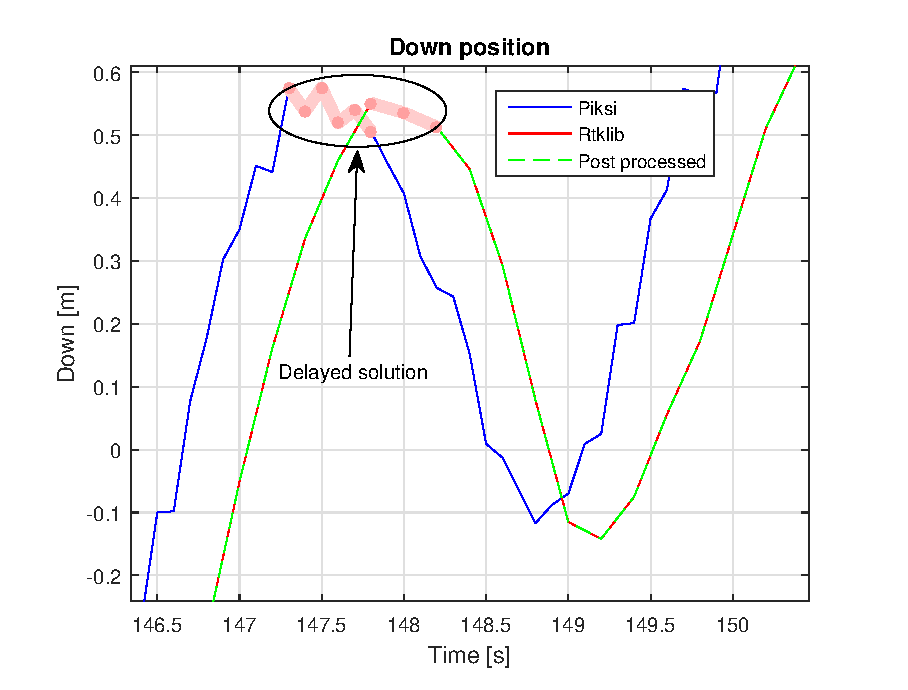
\includegraphics[width=0.7\textwidth]{figs/plots/downDelay.eps}
		\caption{Enhanced Down plot from the first test}
		\label{figure:DownDelay}
\end{figure}
\paragraph{Summary}

Given that the error given in figure \ref{figure:errorPiksiwalk1} and \ref{figure:errorRTKwalk1} is never has a greater absolute value then $0.2m$ it's possible to assume that the true error will be bellow $1m$ which was given as an evasion criterion in the MSc thesis by \citep{Froelich}, if the \gls{rtk-gps} system has a fixed integer ambiguity solution.

\section{Test 1 - Walk test 2}
The second session was performed few minutes after the first, with the same weather condition.
During the second session the Piksi lost its fixed integer ambiguity solution, while \gls{rtklib} managed to keep its fixed integer ambiguity solution as seen in figure \ref{figure:xyWalk2} and \ref{figure:downWalk2}.

\begin{figure}[H]
\begin{subfigure}[H]{1\textwidth}
	\centering
		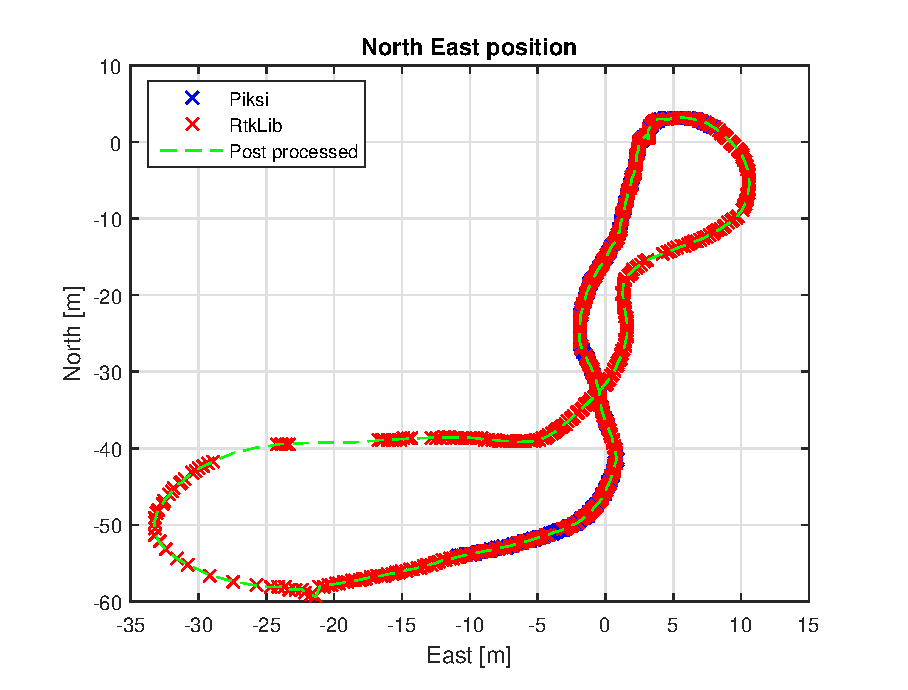
\includegraphics[width=0.7\textwidth]{figs/plots/xywalk2.eps}
		\caption{The North/East position with fixed integer ambiguity solution during the second test}
		\label{figure:xyWalk2}
\end{subfigure}
%\end{figure}
%\begin{figure}[H]
\begin{subfigure}[H]{1\textwidth}
	\centering
		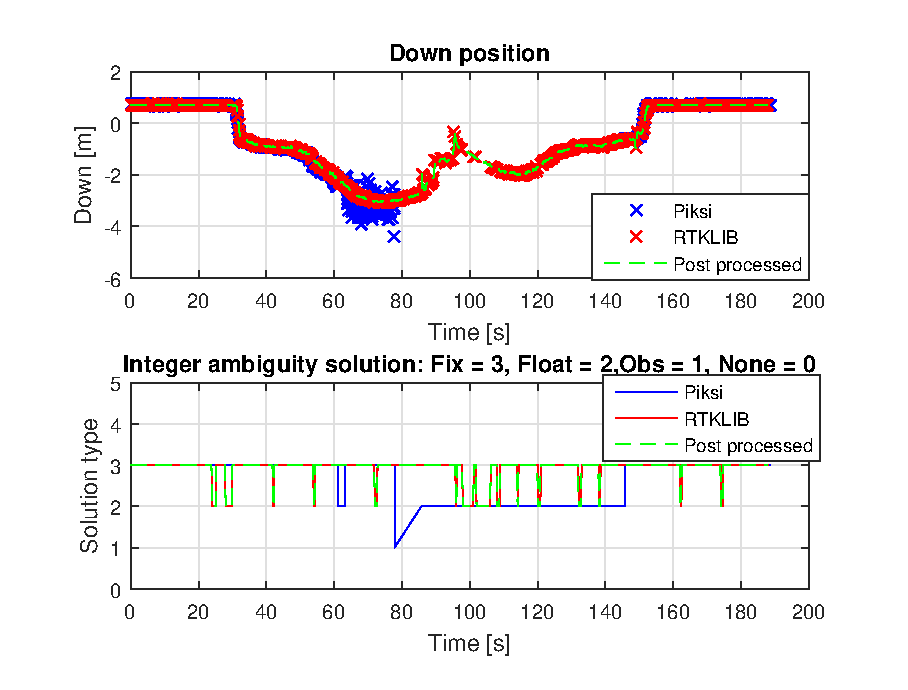
\includegraphics[width=0.7\textwidth]{figs/plots/downWalk2.eps}
		\caption{The Down position and integer ambiguity solution during the second test}
		\label{figure:downWalk2}
\end{subfigure}

\end{figure}
The reason for why the Piksi lost its fixed solution might be because it lost track of several satellite, as seen in figure \ref{figure:numSatWalk2}. Since both receivers share the same antenna it can be concluded that the satellite tracing performance in the Ublox is superior to the Piksi.  Even when the Piksi managed to regain track of the satellite it lost, it took 60 seconds before it regain a fixed integer solution. 
\begin{figure}[H]
	\centering
		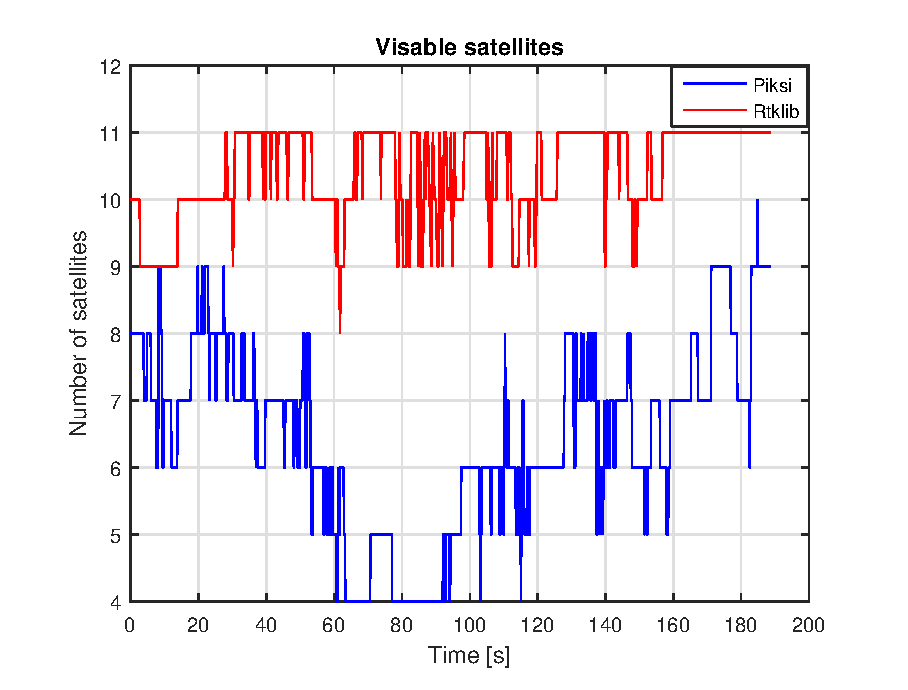
\includegraphics[width=0.7\textwidth]{figs/plots/numSatWalk2.eps}
		\caption{Number of visible satellites in the first test}
		\label{figure:numSatWalk2}
\end{figure}
\section{Flight test}
A flight test with the \gls{uav} was performed at Udduvoll. Because of bad weather only one flight test was performed. Prior to take-of only the \gls{rtklib} was able to provide a fixed integer ambiguity solution. Hence only performance from the \gls{rtklib} is considered in this test, as a navigation system must have a fixed solution before the automatic net landing system can start.

\paragraph{Integer ambiguity solution}~\\

During the flight test the integer ambiguity solution were more float then fixed as seen in figure \ref{figure:DownFlight} and \ref{figure:NorthEastFlight}, which affected the measurement. The same behaviour will be seen during the landing, however if the float solution is accurate enough the system should be able to perform an automatic landing.
\begin{figure}[H]
	\centering
		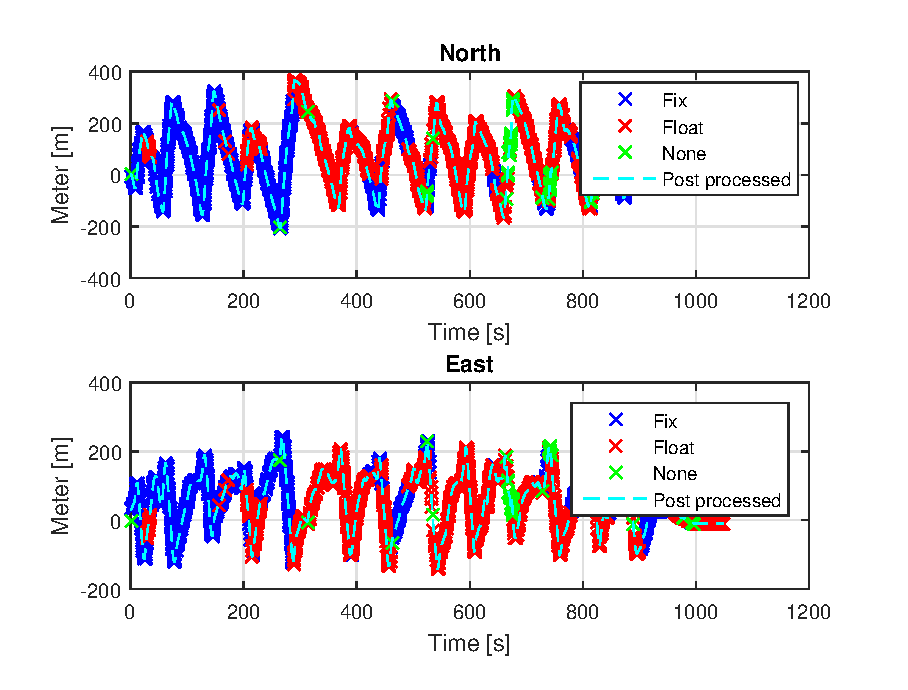
\includegraphics[width=0.7\textwidth]{figs/plots/northEastFlight.eps}
		\caption{The North and East position during the flight}
		\label{figure:NorthEastFlight}
\end{figure}
\begin{figure}[H]
	\centering
		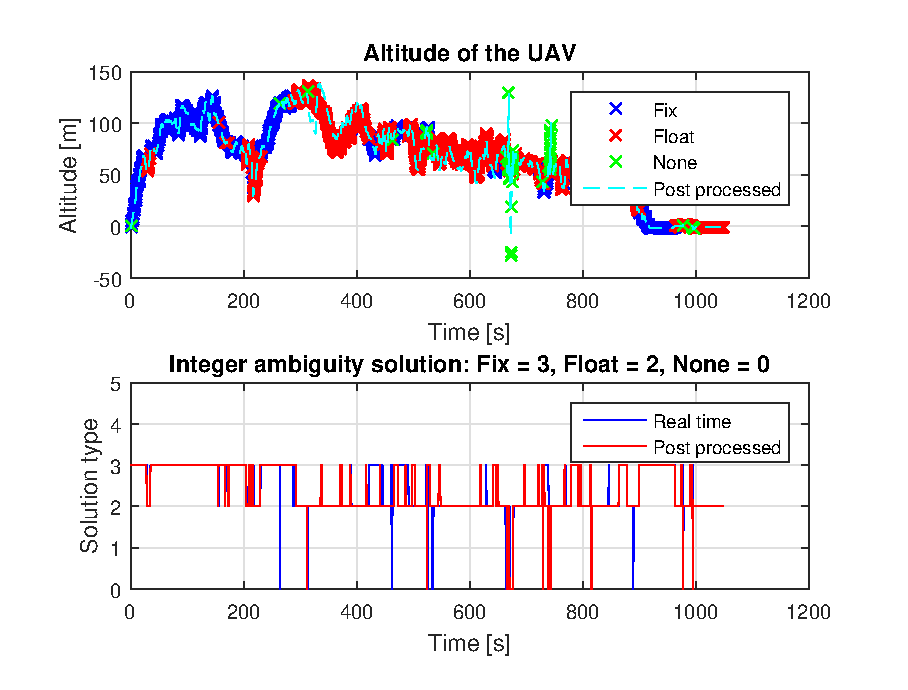
\includegraphics[width=0.7\textwidth]{figs/plots/AltitudeFlight.eps}
		\caption{The altitude during the flight}
		\label{figure:DownFlight}
\end{figure}
\paragraph{Satellite tracking}~\\

The main reason for the lost fixed solution is because of the number of valid satellite the receiver can track experience large variation, as seen i figure \ref{figure:numSatFlight}. A problem experienced during the flight is that large roll and pitch angel of the \gls{uav} puts the antennas in shadow zones, i.e. lose communication with different satellites. That is a problem that can be solved in a control system by setting constraints on the dynamical behaviour of the \gls{uav} especially before and during landing.
\begin{figure}[H]
	\centering
		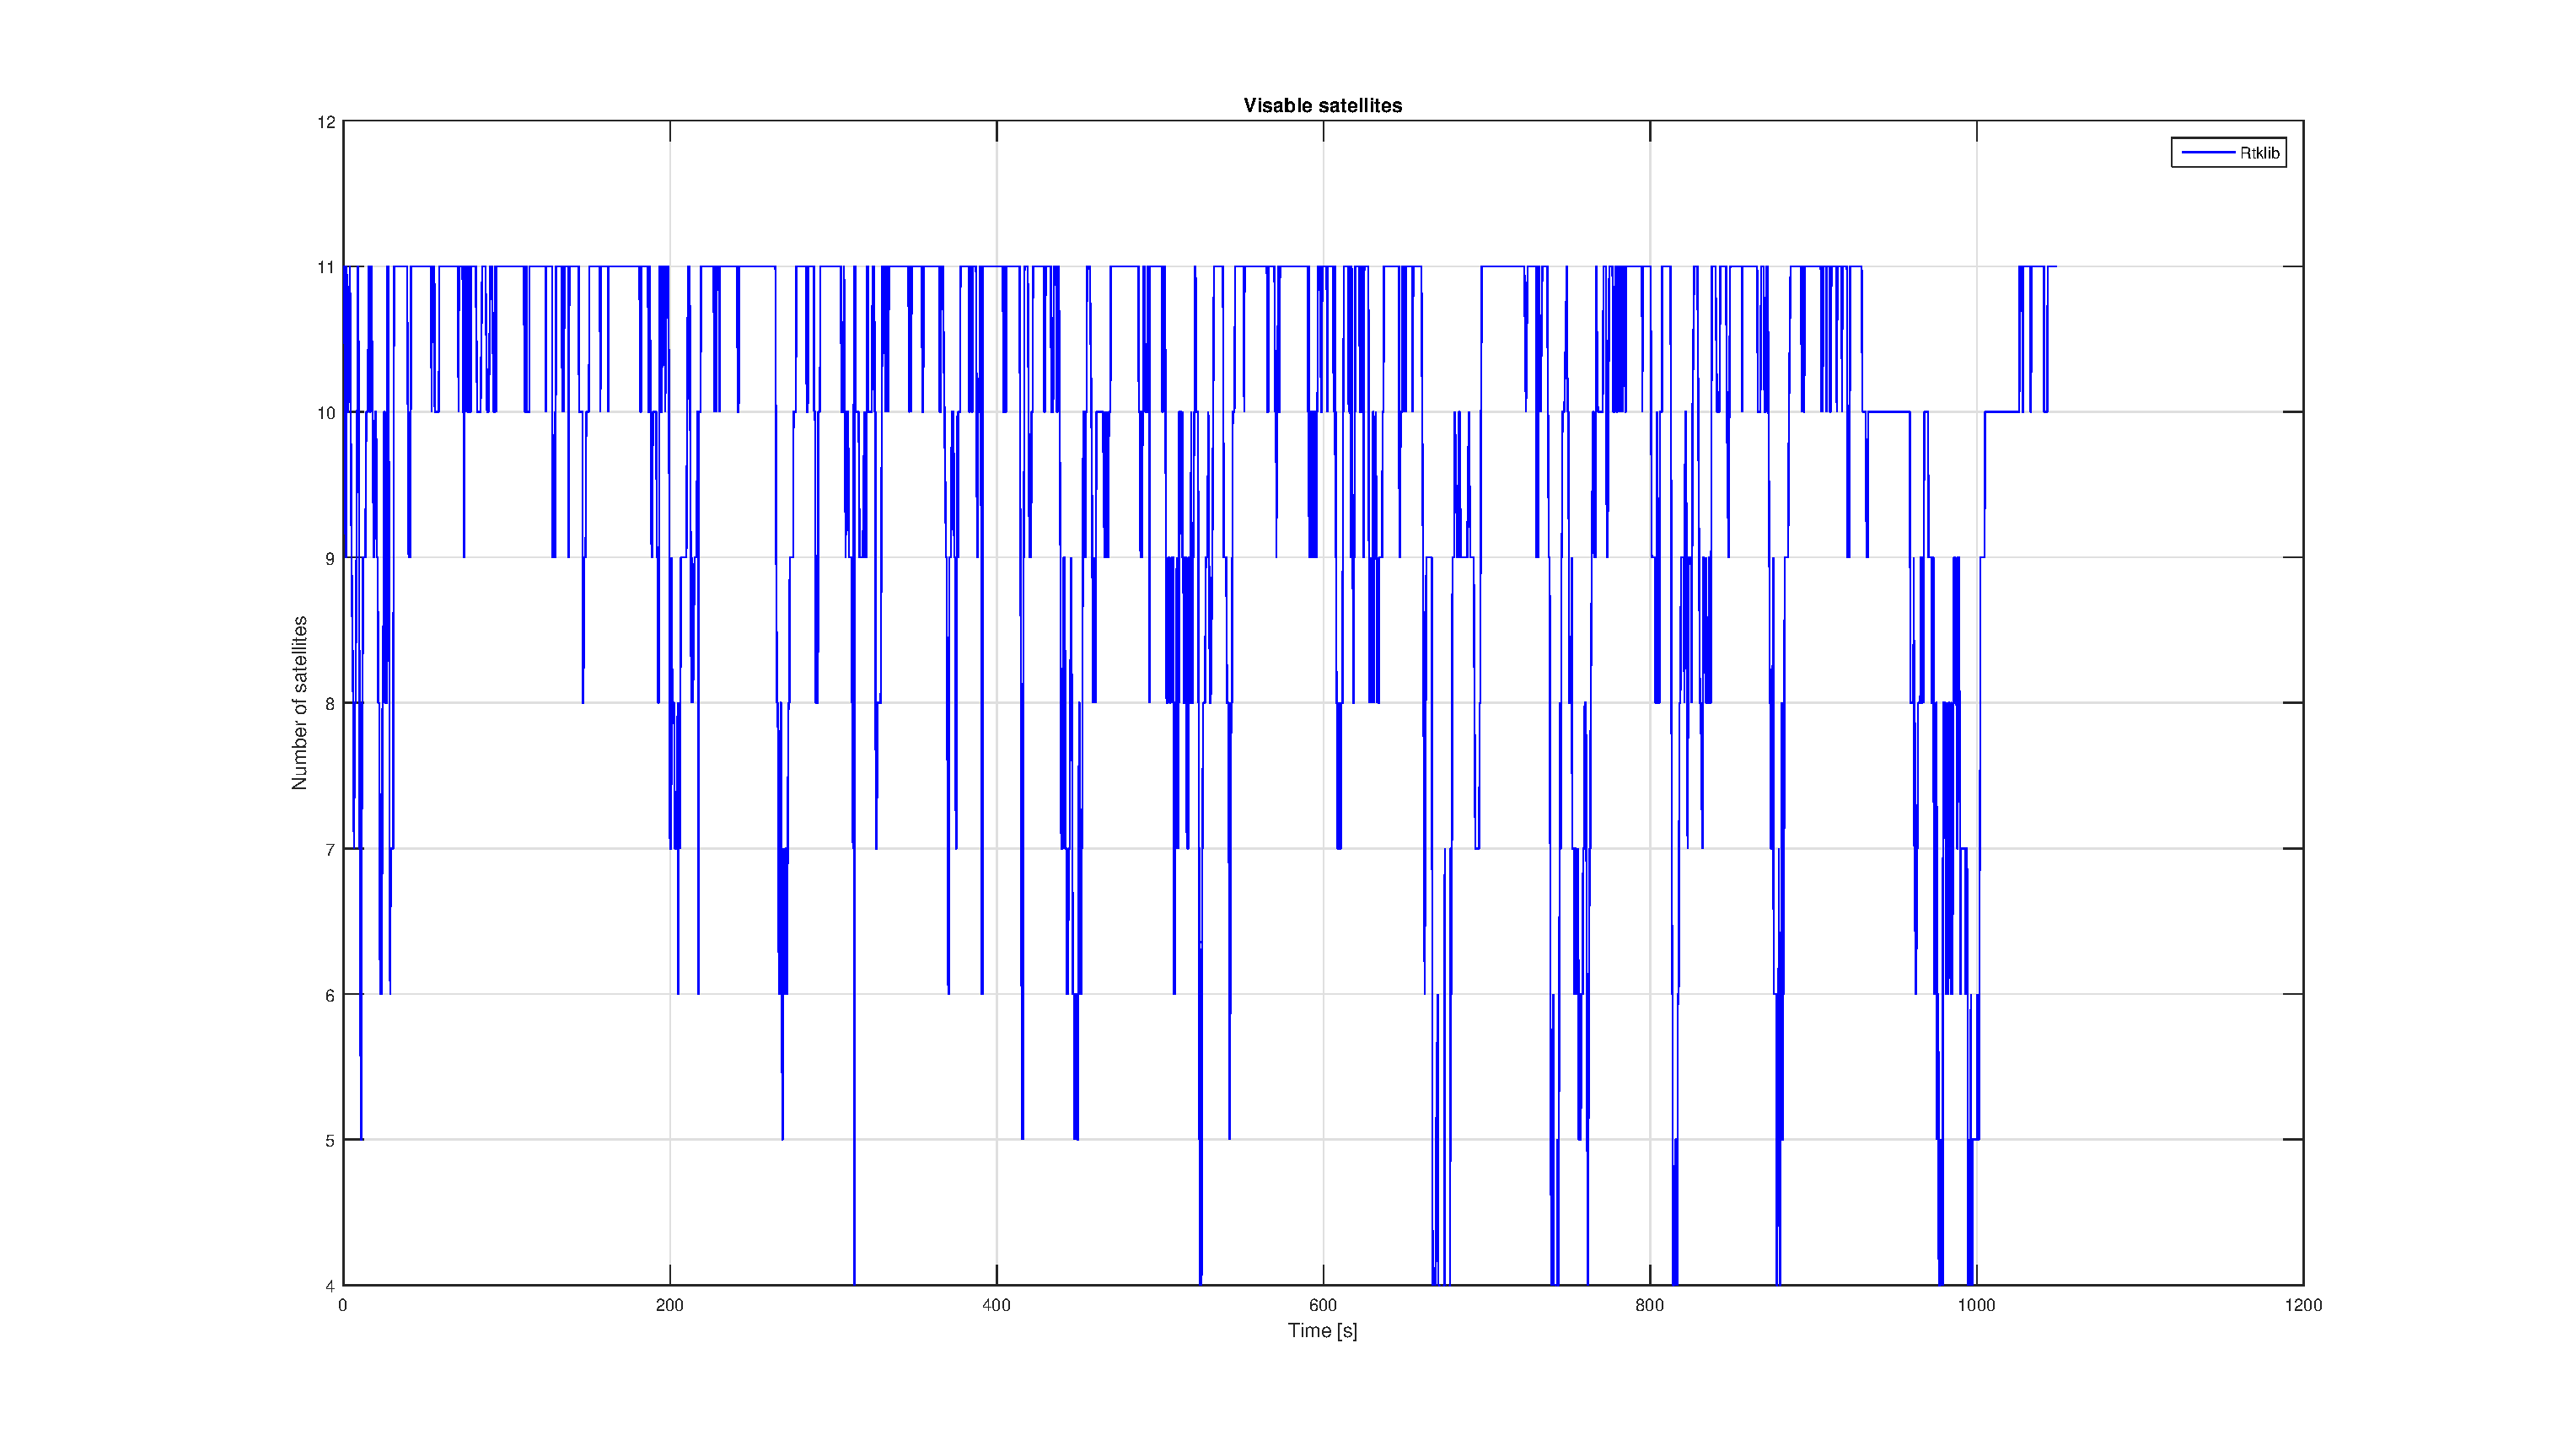
\includegraphics[width=0.7\textwidth]{figs/plots/numSatFlight.eps}
		\caption{Number of visible satellites during the flight}
		\label{figure:numSatFlight}
\end{figure}
%\begin{figure}[H]
%	\centering
%		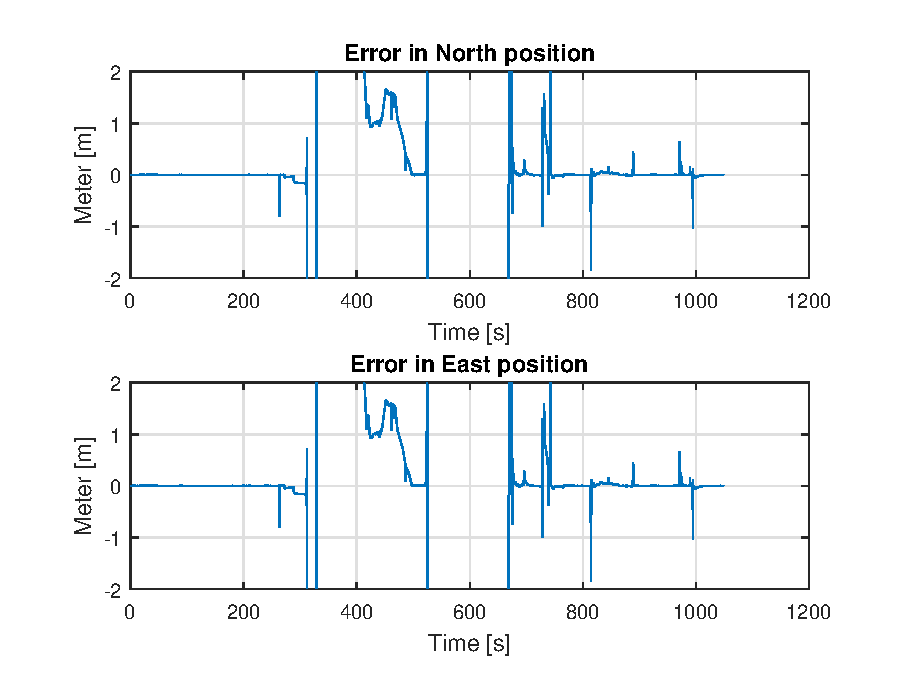
\includegraphics[width=0.7\textwidth]{figs/plots/errorNorthEastFlight.eps}
%		\caption{Velocity data from the piksi and rtklib real time solution}
%		\label{figure:errorNorthEastFlight}
%\end{figure}
%\begin{figure}[H]
%	\centering
%		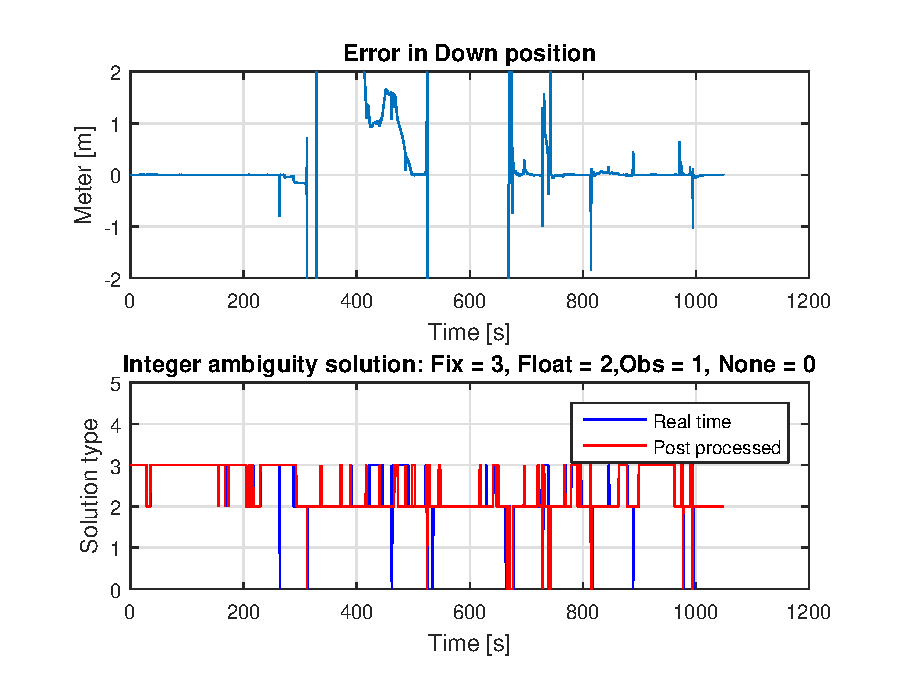
\includegraphics[width=0.7\textwidth]{figs/plots/errorDownFlight.eps}
%		\caption{Velocity data from the piksi and rtklib real time solution}
%		\label{figure:errorDownFlight}
%\end{figure}
\paragraph{Landing}~\\
As expected the navigation system had problem with keeping it's fixed integer solution. The \gls{rtk-gps} position estimate of the landing path is shown in figure \ref{figure:landingPath}. The system kept changing between float and fixed solution during the landing phase. The Down position, in addition to the integer ambiguity solution for the landing phase is seen in \ref{figure:landingDownFlight}. The navigation system was unable to maintain a fixed solution, however it did maintain a float solution and recovered its fixed solution before touch down.
\begin{figure}[H]
	\centering
		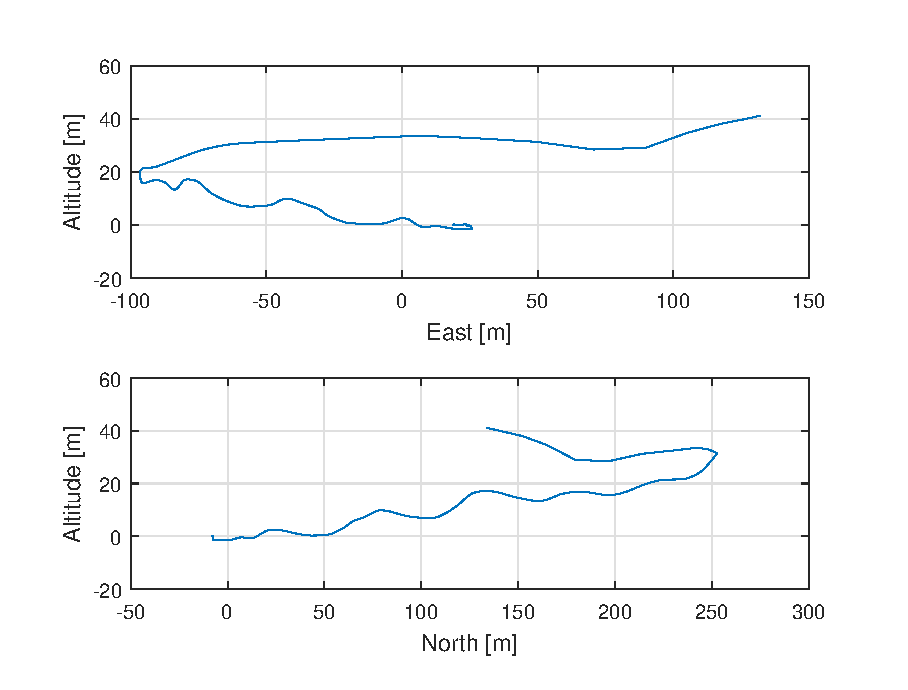
\includegraphics[width=0.7\textwidth]{figs/plots/landingPath.eps}
		\caption{The landing path}
		\label{figure:landingPath}
\end{figure}
\begin{figure}[H]
	\centering
		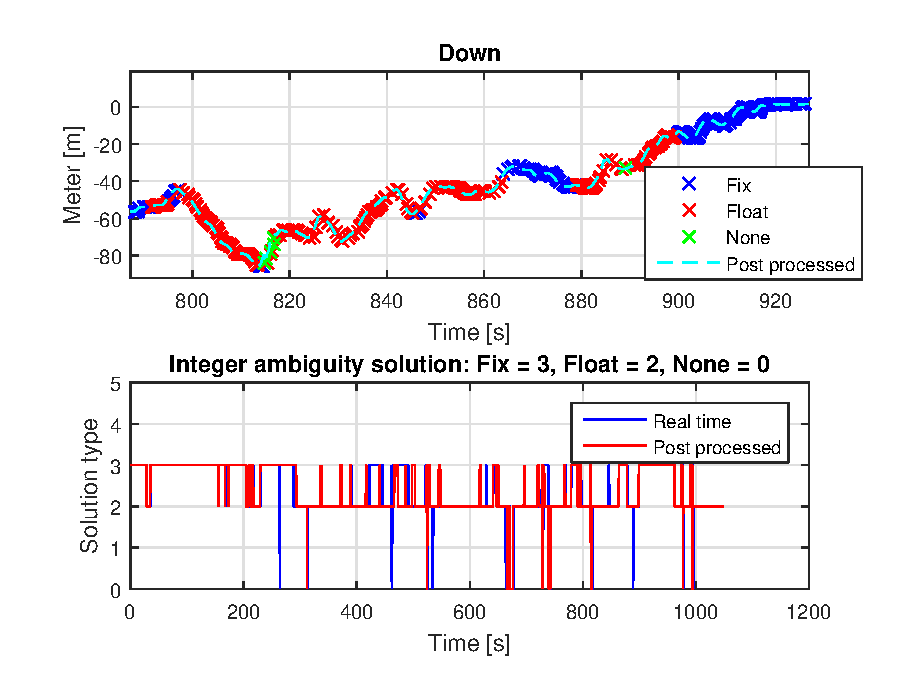
\includegraphics[width=0.7\textwidth]{figs/plots/landingDownFlight.eps}
		\caption{The altitude during the landing}
		\label{figure:landingDownFlight}
\end{figure}

From the error plot seen in figure \ref{figure:landingErrorNorthEastDownFlight} the navigation system was able to estimate its own position with an error bellow 1 meter most of the time. However this is compared to the post processed estimate, which also will diverge from the true value since it is based on the same raw data as the real time solution.

\begin{figure}[H]
	\centering
		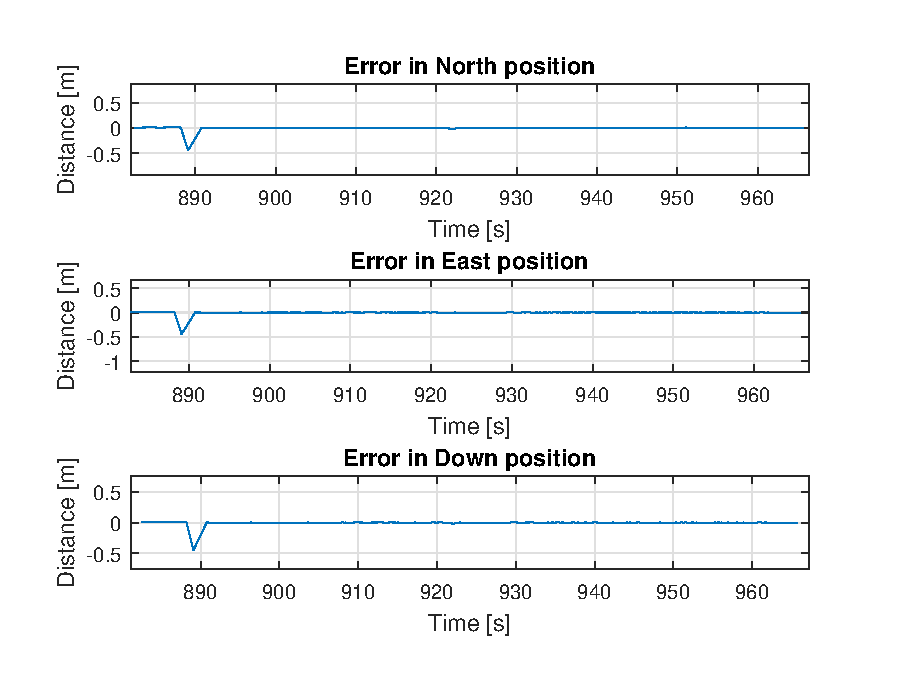
\includegraphics[width=0.7\textwidth]{figs/plots/landingErrorNorthEastDownFlight.eps}
		\caption{The error during the landing}
		\label{figure:landingErrorNorthEastDownFlight}
\end{figure}
The landing velocity seen in figure \ref{figure:landingVelocity} confirms the precision in the estimate that was seen in the first test. However the altitude velocity is less noisy then in figure \ref{figure:VelocityWalk1}, and can be used in a control system.
\begin{figure}[H]
	\centering
		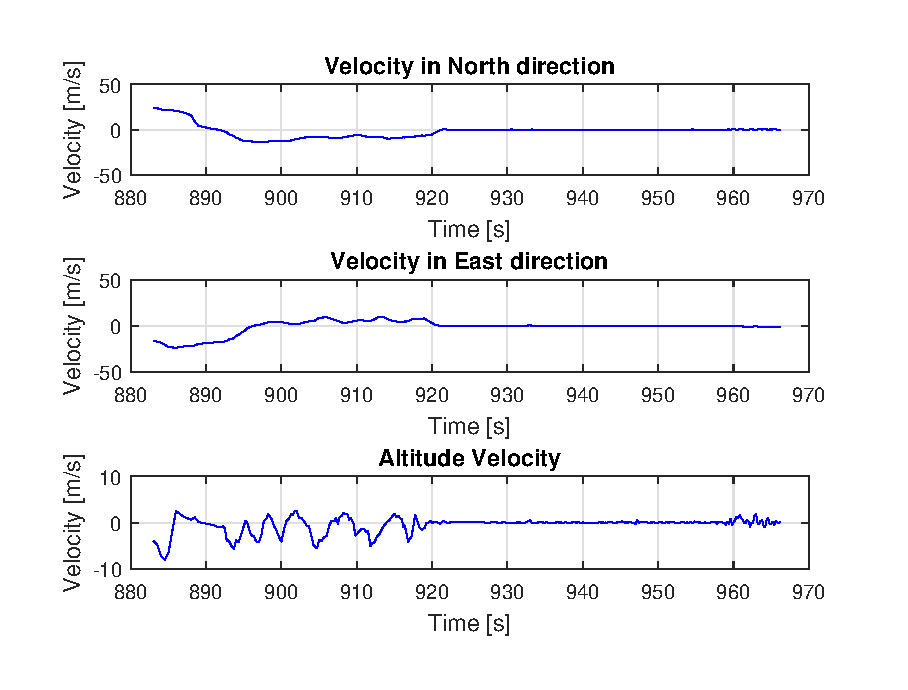
\includegraphics[width=0.7\textwidth]{figs/plots/landingVelocity.eps}
		\caption{The velocity during the landing}
		\label{figure:landingVelocity}
\end{figure}
\cleardoublepage